\documentclass[12 pt, a4paper]{article}% тип документа, размер шрифта
\usepackage{cmap}	
\usepackage{hyperref}
\hypersetup{
    colorlinks=true,
    linkcolor=blue,
    urlcolor=blue,
}
\usepackage{mathtext}
\usepackage[T2A]{fontenc}%поддержка кириллицы в ЛаТеХ
\usepackage[utf8]{inputenc}%кодировка
\usepackage[english,russian]{babel}
\usepackage{indentfirst}

\usepackage{amsmath,amsfonts,amssymb,amsthm,mathtools} % AMS
\usepackage{amsmath}%удобная вёрстка многострочных формул, масштабирующийся текст в формулах, формулы в рамках и др.
\usepackage{amsfonts}%поддержка ажурного и готического шрифтов — например, для записи символа {\displaystyle \mathbb {R} } \mathbb {R} 
\usepackage{amssymb}%amsfonts + несколько сотен дополнительных математических символов
\frenchspacing%запрет длинного пробела после точки
\usepackage{setspace}%возможность установки межстрочного интервала
\usepackage{indentfirst}%пакет позволяет делать в первом абзаце после заголовка абзацный отступ
\onehalfspacing%установка полуторного интервала по умолчанию
\usepackage{graphicx}%подключение рисунков
\graphicspath{{images/}}%путь ко всем рисункам
\usepackage{caption}
\usepackage{float}%плавающие картинки
\usepackage{tikz} % это для чудо-миллиметровки
\usepackage{pgfplots}%для построения графиков
\pgfplotsset{compat=newest, y label style={rotate=-90},  width=10 cm}%версия пакета построения графиков, ширина графиков
\usepackage{pgfplotstable}%простое рисование табличек
\usepackage{lastpage}%пакет нумерации страниц
\usepackage{comment}%возможность вставлять большие комменты
\usepackage{python}%питончик
\usepackage{float}
%%%%% ПОЛЯ
\setlength\parindent{0pt} 
\usepackage[top = 2 cm, bottom = 2 cm, left = 1.5 cm, right = 1.5 cm]{geometry}
\setlength\parindent{0pt}
%%%%% КОЛОНТИТУЛЫ
\usepackage[shortlabels]{enumitem}

\usepackage{fancybox, fancyhdr}
\pagestyle{fancy} 
\fancyhead[L]{Легких Никита Б05-301}
\fancyhead[C]{2.1.3}
% ЛЮБАЯ ДОПОЛНИТЕЛЬНАЯ ИНФОРМАЦИЯ
\fancyfoot[R]{ФПМИ МФТИ}
\renewcommand{\footrulewidth}{0.3 mm}
 

\usepackage{graphicx}
\graphicspath{{pictures/}}
\DeclareGraphicsExtensions{.pdf,.png,.jpg}
\usepackage{wrapfig}
%%% Заголовок
%%% Новые команды
\newcommand{\z}[2]{{{\vspace{0.6cm} \textbf{{Задача {#1}}} \textit{{#2}\\ }}} }
\newcommand{\otv}{{\vspace{0.3cm} \textbf{Ответ: }}}
\newcommand{\uk}{\underline{\textit{Указание.}} }
\newcommand{\prim}{\underline{\textit{Примечание.}} }
\newcommand{\sol}[1]{{{\vspace{0.3cm} \textbf{{Задача {#1}} }\\ }}}



\begin{document} % конец преамбулы, начало документа

\begin{center}
\section*{Работа №2.1.3}
    \section*{Определение $C_p/C_\upsilon$ по скорости звука в газе}
\end{center}
\textbf{Цель работы:} 1) измерение частоты колебаний и длины волны при резонансе звуковых колебаний в газе, заполняющем трубу; 2) определение показателя адиабаты с помощью уравнения состояния идеального газа.
 \\ \\
\textbf{В работе используются:} звуковой генератор ГЗ; электорнный осциллограф ЭО; микрофон; телефон; теплоизолированная труба, обогреваемая водой из термостата; теплоизолированная труба без термостата; баллон со сжатым углекислым газом; газгольдер.


\section*{Теоретическая справка}
Один из наиболее точных методов измерения показателя адиабаты $\gamma$ основан на зависимости от него скорости распространения звуковой волны в газе. Последняя в газах определяется формулой $c = \sqrt{\frac{\gamma RT}{\mu}}$, из которой можно выразить показатель адиабаты:
 	\begin{equation}\label{1}
 	\gamma = \frac{\mu}{RT}c^2,
 	\end{equation}
где $T$ --- температура газа, $\mu$ --- его молярная масса, а $R$ --- газовая постоянная. \\
Скорость $c$ звука связана с его частотой $f$ и длиной волны $\lambda$ соотношением
	\begin{equation}
	c = \lambda f.
	\end{equation}
С волнами в трубке удобнее всего работать при резонансе. Условие резонанса выглядит как
	\begin{equation}
	L = n\frac{\lambda}{2},
	\end{equation}
где $L$ --- длина трубки, $\lambda$ --- длина волны, $n$ --- целое число.\\
В данной работе при постоянной длине трубки изменяется частота звуковых колебаний $f$, а с ней и длина звуковой волны $\lambda$. Для последовательных резонансов можно записать:
	\begin{equation}
	L = n\frac{\lambda_1}{2} = (n + 1)\frac{\lambda_2}{2} = ... = (n + k)\frac{\lambda_{k + 1}}{2}
	\end{equation}
С учётом (2) имеем
	\begin{equation}
	f_{t+1} = \frac{c}{\lambda_{t+1}} = f_1 + \frac{c}{2L}t~ (t = 0, 1,..., k)
	\end{equation}
Таким образом, $c/2L$ можно найти как угловой коэффициент графика зависимости частоты от номера резонанса.
\section*{Установка}
В работе мы будем использовать две похожие, но все же различные установки: \\
\textbf{Первая}, 
Схема установки, используемой в работе приведена на рисунке ниже
\begin{figure}[h]
\centering
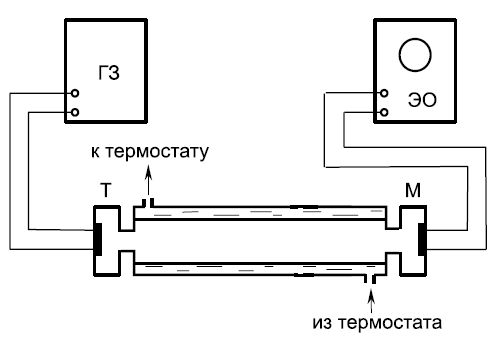
\includegraphics[width=0.5\linewidth]{1.png}
\label{fig:mpr}
\end{figure}
Звуковые колебания в трубе возбуждаются телефоном Т и улавливаются микрофоном М. Мембрана телефона приводится в движение переменным током звуковой частоты. В качестве источника переменной ЭДС используется звуковой генератор ГЗ. Возникающий в микрофоне сигнал возникает на экране осциллографа ЭО. \\
Микрофон и телефон присоединены к установке через тонкие резиновые трубки. Такая связь достаточна для возбуждения и обнаружения звуковых колебаний в трубе и в то же время мало возмущает эти колебания: при расчетах оба конца трубы можно считать неподвижными, а влиянием соединительных отверстий пренебречь. \\
Установка содержит теплоизолированную трубу постоянной длины. Воздух в трубке нагревается водой из термостата. Температура газа принимается равной температуре омывающей трубу воды. \\
\textbf{Вторая},
Установка схожа с первой, только к трубе подключен не термостат а газгольдер, позволяющий менять состав газа находящийся внутрее нее.
\section*{Задание}
\begin{enumerate}
    \item Снимаем комнатную температуру: $$T_к = 24.5^oC, \;L = 795 мм.$$ Включаем в сеть ЭО и ГЗ, даём им прогреться 5 минут. Включаем на осциллографе тумблер <<луч>> и ручками управления добиваемся прямой линии на экране. Устанавливаем нуль на звуковом генераторе.
    \item Подбираем напряжение на выходе генератора так, чтобы амплитуда колебаний при резонансе была достаточно велика, возьмем значение $U_{выходное} = 20\; В$
    \item Начнем с измерений на второй установке с трубкой заполненной воздухом, для этого возьмем примерное значение скорости звука в воздухе $c = 300\;м/с$, и расчитаем примерное значение $f_1 = 188.7\;Гц$. Далее произведем измерения вблизи данного значени и потом будем умножать результат на натуральные числа в поисках других обертонов. Потом проделываем тоже самое для трубки заполненной $CO_2$
    \begin{center}
    \begin{tabular}{|c|c|c|}
    \hline
    $t$ &  $f_{воздух}$  & $f_{CO_2}$\\ \hline
    1   & 198.4 & 176.0\\ \hline
    2   & 390.2 &341.5\\ \hline
    3   & 581.4 &503.2\\ \hline
    4   & 781.8 &675.5\\ \hline
    5   & 972.3 &842.4\\ \hline
    \end{tabular}
    \end{center}
    График $f_{воздух}$ от $n$
    \begin{figure}[h]
    \centering
    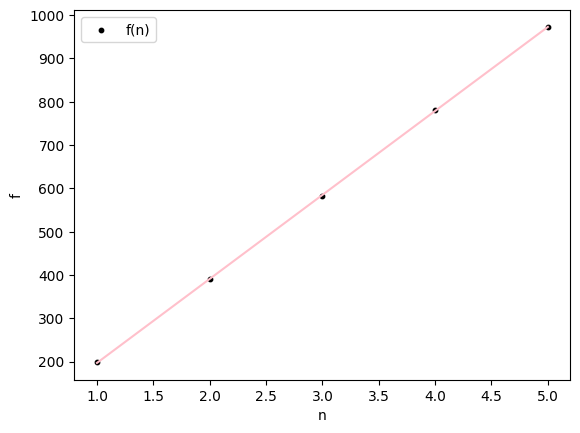
\includegraphics[width=0.55\linewidth]{2.1.3/first.png}
    \label{fig:mpr}
    \end{figure} \\
    График $f_{CO_2}$ от $n$
    \begin{figure}[h]
    \centering
    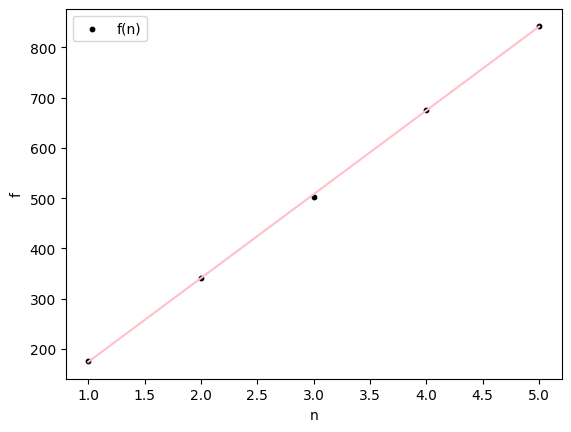
\includegraphics[width=0.55\linewidth]{2.1.3/second.png}
    \label{fig:mpr}
    \end{figure} \newpage
    С помощью метода МНК получаем следующие значения: 
    $$k_{воздуха} = (193.9\pm0.8)\;с^{-1} \rightarrow c_{воздуха} = k_{воздуха}\cdot2\cdot L = (308.3\pm1.2) \;м/с$$
    $$k_{CO_2} = (166.7\pm0.8)\;с^{-1} \rightarrow c_{CO_2} = k_{CO_2}\cdot2\cdot L = (265.1\pm1.0) \;м/с$$
    Видно что давнные значения недалеки от истины. \\
    \item Получив примерные значения скорости звука в исследуемой среде (воздухе), приступаем ко второй части эксперимента, то есть с первой установкой. $L = 800\;мм$\\
    Измерим скорость звука при $T = 23^oC = 296\;К$ \\
    \begin{center}
    \begin{tabular}{|c|c|}
    \hline
   $k$ & $f_{k+1} - f_{k}$ \\ \hline
    1 & 102                   \\ \hline
    2 & 249                   \\ \hline
    3 & 461                   \\ \hline
    4 & 669                   \\ \hline
    5 & 1109                  \\ \hline
    \end{tabular}
    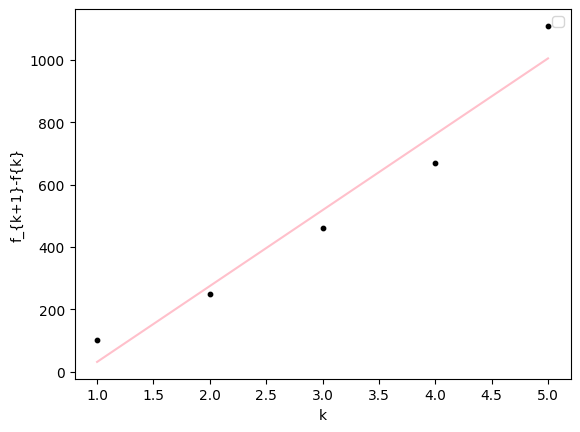
\includegraphics[width=0.6\linewidth]{2.1.3/t1.png}
    \end{center}
    Отсюда: $k = (234\pm54) c^{-1} \rightarrow c = k\cdot2\cdot L = (375\pm86)\;м/с$, заметим что погрешность очень велика, но если убрать последнюю точку, то получим: $k = (191.3\pm15.1) c^{-1} \rightarrow c = (306.1\pm24.1)\;м/с$, здесь относительная погрешность поменьше и данному результату я склонен верить больше. \newpage
    Теперь при $T = 34.5^oC = 307.7\;К$ \\
    \begin{center}
    \begin{tabular}{|c|c|}
    \hline
   $k$ & $f_{k+1} - f_{k}$ \\ \hline
    1 & 102                   \\ \hline
    2 & 249                   \\ \hline
    3 & 461                   \\ \hline
    4 & 669                   \\ \hline
    5 & 1109                  \\ \hline
    \end{tabular}
    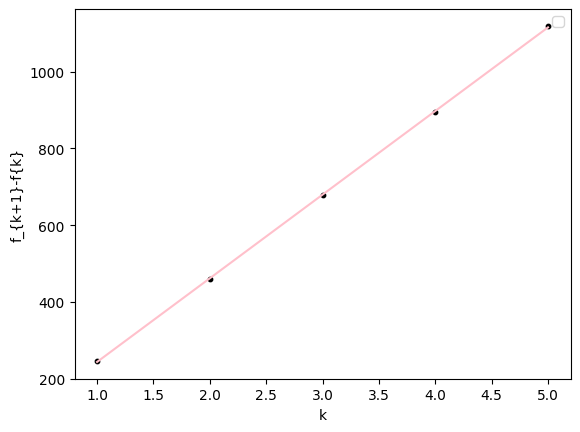
\includegraphics[width=0.6\linewidth]{2.1.3/t2.png}
    \end{center}
    Отсюда: $k = (217.9\pm1.2) c^{-1} \rightarrow c = k\cdot2\cdot L = (347.2\pm2.0)\;м/с$, такое значение гораздо лучше чем с прошлой температурой, оставляем его. \\
    Теперь при $T = 50^oC = 323.2\;К$ \\
    \begin{center}
    \begin{tabular}{|c|c|}
    \hline
   $k$ & $f_{k+1} - f_{k}$ \\ \hline
    1 & 214                   \\ \hline
    2 & 436                   \\ \hline
    3 & 662                   \\ \hline
    4 & 887                   \\ \hline
    5 & 1110                  \\ \hline
    \end{tabular}
    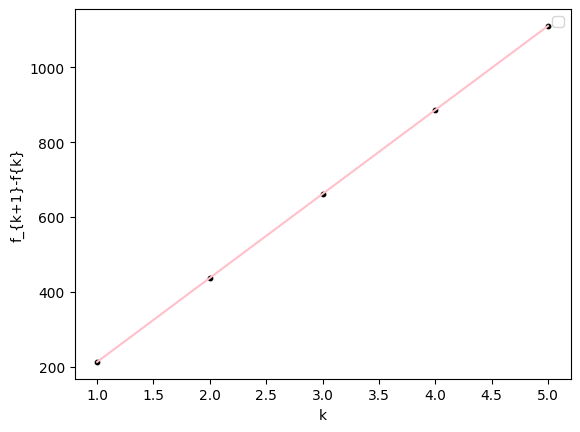
\includegraphics[width=0.6\linewidth]{2.1.3/t3.png}
    \end{center}
    Отсюда: $k = (224.3\pm0.4) c^{-1} \rightarrow c = k\cdot2\cdot L = (358.9\pm0.6)\;м/с$. \newpage
    Теперь при $T = 60^oC = 333.2\;К$ \\
    \begin{center}
    \begin{tabular}{|c|c|}
    \hline
   $k$ & $f_{k+1} - f_{k}$ \\ \hline
    1 & 263                   \\ \hline
    2 & 487                   \\ \hline
    3 & 712                   \\ \hline
    4 & 940                   \\ \hline
    5 & 1118                  \\ \hline
    \end{tabular}
    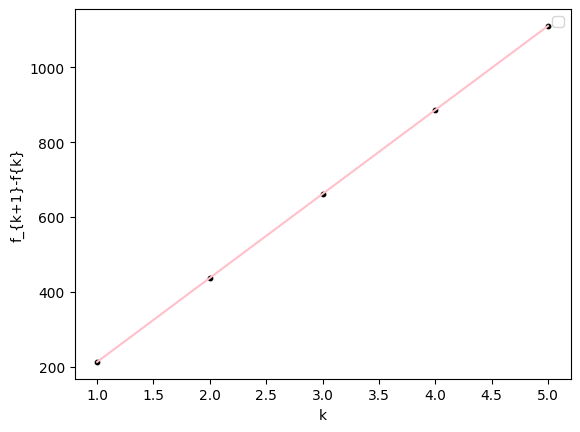
\includegraphics[width=0.6\linewidth]{2.1.3/t3.png}
    \end{center}
    Отсюда: $k = (216.3\pm4.3) c^{-1} \rightarrow c = k\cdot2\cdot L = (346.1\pm7.0)\;м/с$. \\ \\
    Исходя из измерений при разных температурах получаем следующую серию значений: 
    \begin{center}
    \begin{tabular}{|c|c|c|c|c|}
    \hline
    $T$, К & $c,\;м/с$ & $\Delta c,\;м/с$ & $\gamma$& $\Delta \gamma$\\ \hline
    297.65 & 308.3     & 1.2        & 1.11 & 0.01 \\ \hline
    296    & 306.1     & 24.1       & 1.10 & 0.17 \\ \hline
    307.7  & 347.2     & 2          & 1.37 & 0.02 \\ \hline
    323.2  & 358.9     & 0.6        & 1.39 & 0.00 \\ \hline
    333.2  & 346.1     & 7          & 1.25 & 0.05 \\ \hline
    \end{tabular}
    \end{center}
    Вычисление $\gamma$ делалось по формуле \ref{1}, а $\Delta \gamma = \gamma\cdot (2\frac{\Delta c}{c} + \frac{\Delta T}{T}) \approx \gamma\cdot 2\frac{\Delta c}{c}$. \\ \\
    Анализируя таблицу получаем что: $$\gamma = \gamma_{average} = 1.25,$$ $$ \Delta \gamma = \sqrt{\Delta \gamma_{statistic}^2 + \Delta \gamma_{average}^2},\;где$$
    $$\Delta \gamma_{average} = 0.05$$
    $$\Delta \gamma_{statistic} = \sqrt{\frac{\Sigma^5_{i = 1} (\gamma_i - \gamma_{average})^2}{5}} = 0.06 \Rightarrow$$
    $$\Delta \gamma =\sqrt{0.05^2 + 0.06^2} = 0.08$$    
\end{enumerate}

\section*{Вывод}
Мы получили значени $\gamma = (1.25\pm0.08)$, табличное значение: $\gamma_{воздуха} = 1.403$, к сожалению полученное среднее значение не близко к реальному, но вот одно из значений $\gamma = 1.39$ при $T = 323.2\;К$ максимально близкое значение к реальному, плюс оно с наименьшей погрещностью сильно меньшей самого значения. Получается что качественным измерением было только одно.


\end{document}
